\newpage
\section{Branch-and-Bound Technique for Solving Integer Programs}

% Principi dell'algoritmo Branch-and-Bound
\subsection{Principi dell'argoritmo Branch-and-Bound}

I problemi che cerchiamo di risolvere sono \hl{lineari con variabli decisionali}, il problema è che \hl{alcune variabili possono essere intere}, o anche binarie, al posto di essere continue. Per questi casi abbiamo alcuni \hl{approcci naive} da usare:

\begin{enumerate}
    \item \hl{brute force}: se abbiamo n variabili binarie le soluzioni ammissibili sono $2^n$. Andremo quindi a \textbf{generare tutte le soluzioni e verficarne i vincoli} sono soddisfatti (non computazionalmente possibile)
    \item \hl{rounding}: sostituisco le variabili intere con un "rilassamento" del vincolo di integrità. Quindi il problema \textbf{$P$}:
        $$\max z = 3x_1 + 4x_2 - 2x_3 + 3x_4 - 2x_5$$

        con vincoli:
        \begin{itemize}
            \item $2x_1 + 2x_2 + 2x_3 + 2x_4 + 2x_5 \leq 4$
            \item $x_1, x_2, x_3, x_4, x_5 = 0/1$
        \end{itemize}

        diventa \textbf{$R(P)$}:
        $$\max z = 3x_1 + 4x_2 – 2x_3 + 3x_4 – 2x_5$$
        
        con vincoli:
        \begin{itemize}
            \item $2x_1 + 2x_2 + 2x_3 + 2x_4 + 2x_5 \leq 4$
            \item $0 \leq x_1, x_2, x_3, x_4, x_5 \leq 1$
        \end{itemize}
        
        Avremo un \textbf{caso fortunato} se la soluzione di $R(P)$ è anche quella di $P$.

\end{enumerate}


% Approccio Branch-and-Bound
\subsection{Approccio Branch-and-Bound}

È detta tecnica di enumeramerazione parsiale dove \hl{ci si procura una stima del valore della soluzione ottima rilassando il vincolo di integrita'} sulle veriabili intere.

Nella sua risoluzione tramite blackbox potremo avere \hl{4 casistiche}:

\begin{enumerate}
    \item \hl{$R(P)$ inammissibile} $\to$ $P$ inammissibile:
    
        \begin{figure}[H]
        \centering
        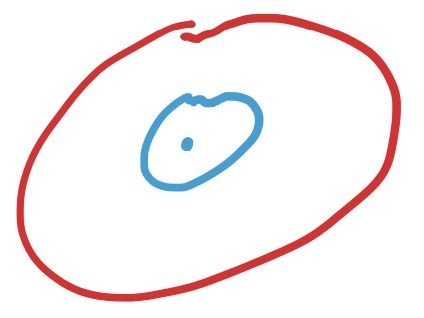
\includegraphics[scale=0.2]{rpp.jpeg}
        \caption{$R(P)$ che contiene $P$} 
        \label{rpp}
        \end{figure}
    
    \item $R(P)$ unbounded $\to$ \hl{$P$ puo' essere unbounded} (dove abbiamo variabili intere):
    
        \begin{figure}[H]
        \centering
        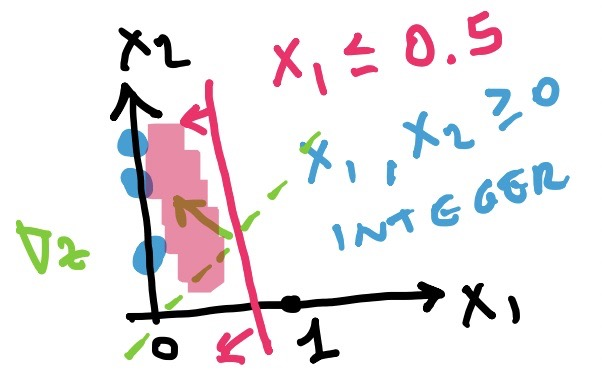
\includegraphics[scale=0.2]{cas1.jpeg}
        \caption{In caso di $P$ unbounded} 
        \label{cas1}
        \end{figure}
    
    \item $R(P)$ unbounded $\to$ \hl{$P$ puo' essere inammissibile} (dove non abbiamo variabili intere):
    
        \begin{figure}[H]
        \centering
        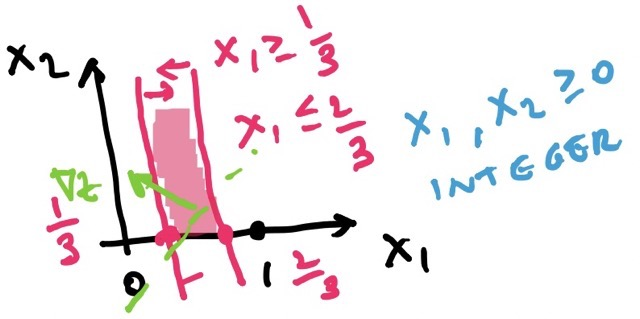
\includegraphics[scale=0.25]{cas2.jpeg}
        \caption{In caso di $P$ inammissibile} 
        \label{cas2}
        \end{figure}

        (p.s: non posso saperlo dato che la blackbox mi sa solo $R(P)$)

    \item \hl{$R(P)$ ha soluzione ottima} $\to$ $P$ inammissibile
        
        \begin{figure}[H]
        \centering
        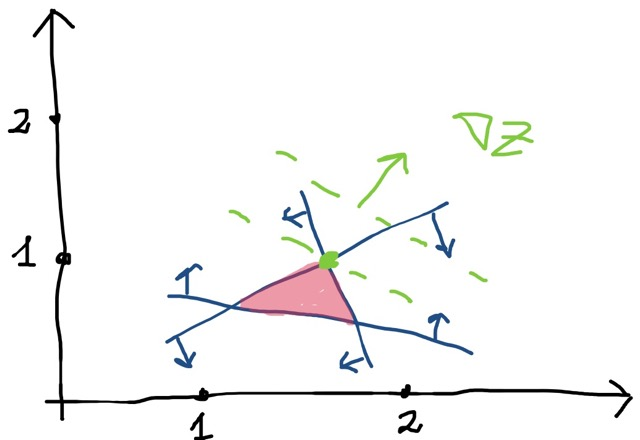
\includegraphics[scale=0.25]{pin.jpeg}
        \caption{$R(P)$ ottima ma $P$ inammissibile} 
        \label{pin}
        \end{figure}

        (p.s: non posso saperlo dato che la blackbox mi sa solo $R(P)$)

    \item \hl{$R(P)$ ha soluzione ottima} $\to$ $P$ ammissibile
        
        \begin{figure}[H]
        \centering
        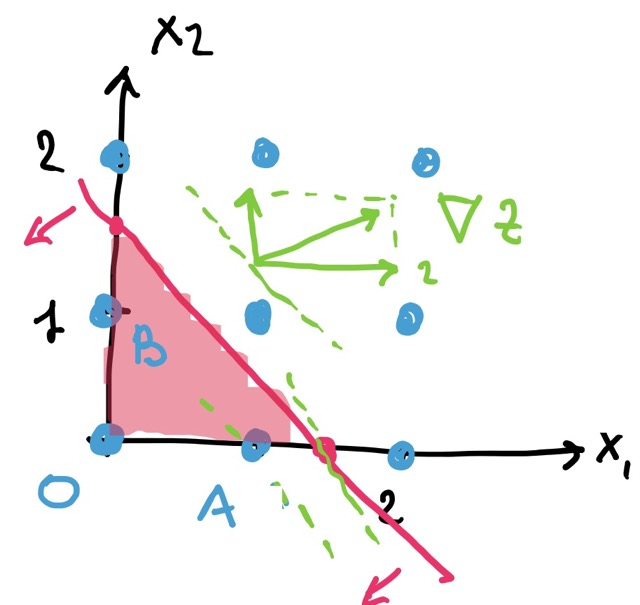
\includegraphics[scale=0.25]{pam.jpeg}
        \caption{$R(P)$ ottima ma $P$ ammissibile} 
        \label{pam}
        \end{figure}

        dove avremo come \textbf{soluzioni intere}:
        $$O(0,0),\ A(1,0),\ B(0, 1)$$

        Andrò allora a \textbf{traslare al curva di livello} fino a trovare la \textbf{soluzione $R(P)$: primo numero ammissibile} nella regione ammissibile, nceve \textbf{per $P$: primo numero intero ammissibile}

\end{enumerate}

La \hl{soluzione ottima di ottimizzazione sara' quella di $R(P)$} di rilassamento continuo, perché \hl{ha meno vincoli} fornendo una soluzione migliore o uguale della nostra stima. Allora se massimizziamo:
$$Z^*_{R(P)} \geq Z^*_P$$

se sto minimizzando:
$$Z^*_{R(P)} \leq Z^*_P$$

dove avrò rispettivamente \hl{upper-bound} e \hl{lower-bound}.


% Branching
\subsection{Branching}

Oltre ad upper-bound e lower-bound su effettua un \hl{branch} cioè una \hl{suddivisione del problema in sottoproblemi}, dove per le soluzioni ammissibili (s.a.):

\begin{itemize}
    \item $P$ s.a. = $P_1$ s.a. $\cup$ $P_2$ s.a.
    \item $P_1$ s.a. $\cap$ $P_2$ s.a. = insieme vuoto
    \item $\underline{x}^*$ $\notin$ $P_1$ s.a., $P_2$ s.a.
\end{itemize}

con $\underline{x}^*$ possibile vincolo applicabile a $x_1$ o $x_2$. Infatti per un problema a 2 variabili abbiamo:

\begin{figure}[H]
\centering
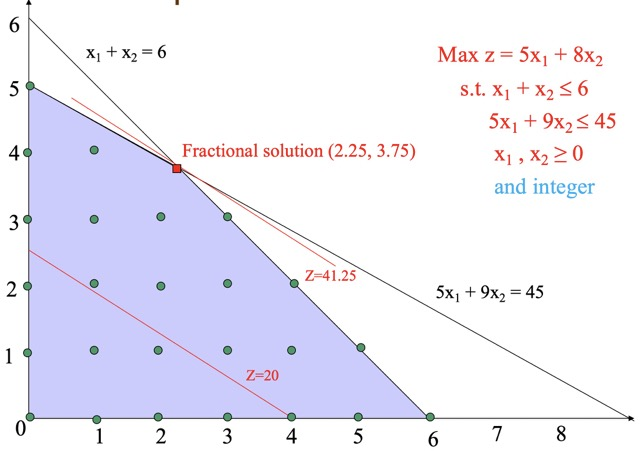
\includegraphics[scale=0.4]{branchprob.jpeg}
\caption{Problema di branching} 
\label{branchprob}
\end{figure}

con soluzione ottima in $(2.25, 3.75)$ con upper: $z = 41.25$.

\hl{Avendo dei valori frazionari effetttuo un branch} per creare dei sottoproblemi. Avendo la soluzione in $(2.25, 3.75)$ allora effettuo il "troncamento" in:
$$x_2 \leq 3,\ x_2 \geq 4$$

\begin{figure}[H]
\centering
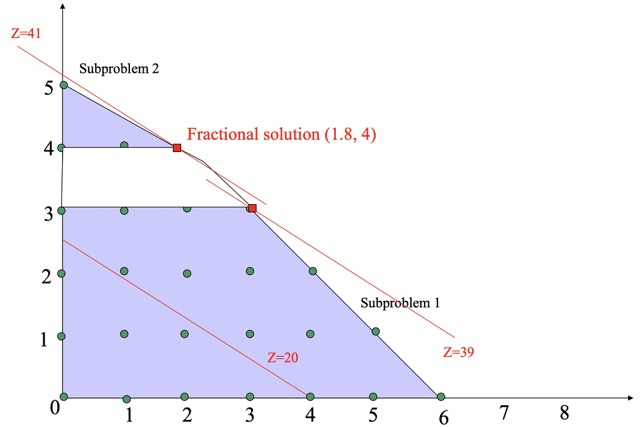
\includegraphics[scale=0.4]{child1.jpeg}
\caption{Primo child} 
\label{child1}
\end{figure}

Quindi per il \hl{sottoproblema $P_1$} con f.o:
$$\max z = 5x_1 + 8x_2$$

e vincoli:
\begin{itemize}
    \item $x_1 + x_2 \leq 6$
    \item $5x_1 + 9x_2 \leq 45$
    \item $x_2 \leq 3$
    \item $x_1,\ x_2 \geq 0$
\end{itemize}

che avrà come \hl{soluzione} $(3, 3)$ con uppeboound $z = 39$.

invece per il \hl{sottoproblema $P_2$} con f.o:
$$\max z = 5x_1 + 8x_2$$

e vincoli:
\begin{itemize}
    \item $x_1 + x_2 \leq 6$
    \item $5x_1 + 9x_2 \leq 45$
    \item $x_2 \geq 4$
    \item $x_1,\ x_2 \geq 0$
\end{itemize}

che avrà come \hl{soluzione} $(1.8, 4)$ con uppeboound $z = 41$.

Avendo \hl{numeri interi in $P_1$} ho una soluzione ottima e non dovrò fare branch su $P_1$ e dato il suo valore di $z$ che è \hl{cerco in $P_2$} con f.o:
risolveremo allora risolvendo il sottoproblema 1 con soluzione 3, 3 con z = 39 allora non ho bisogno di eplorare ancora dato che ho già la soluzione ottima \hl{minore di quello di $P_2$} allora: \hl{scarto $P_1$ e continuo i branch su $P_2$}.


\begin{figure}[H]
\centering
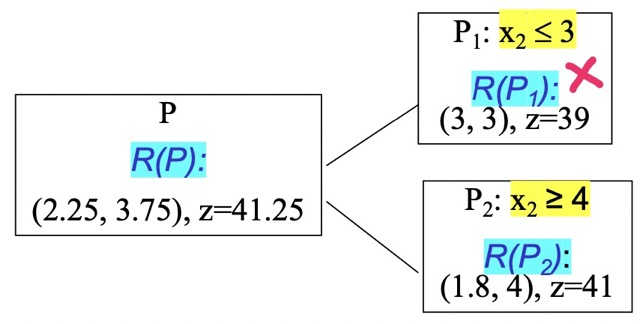
\includegraphics[scale=0.4]{nop1.jpeg}
\caption{Scarto del primo child} 
\label{nop1}
\end{figure}


Effettuando il branch avremo con $P_3$ che ha  $x_1 \leq 1$ e $P_4$ che ha $x_1 \geq 2$

risolviamo i loro rilassamenti 

tenendo in conto che i child ereditano i vincoli del parent


avremo che $R(P_4)$ è inammissibile allora anche P lo sarà
invece per $P_3$ abbiamo che $R(P_3)$ avrà $(1, 4.44)$ con $z = 40.55$

allora continuamo con il branch ed avremo:

$P_5 x_2 \leq 4$ con $(1, 4)$ con $z = 37$
$P_6 x_2 \geq 5$ con $(0, 5)$ con $z = 40$

scartiamo allora $P_5$ che ci fa arrivare ad un massimo di 37 < 40 di $P_6$

abiamo allora che non ci sono piu branch da creare.

fathoming: posso eliminare un sottoprob se

- il rilassmento suo è inammissible
- il rilassamento di $P$ ($R(P)$) ha soluzione ottima intera, allora è anche osluzione di $P$
- fenomeno di dominanza: una $z$ è più grande delle altre


per scrivere lo pseudocodice dobbimao veder come fare branch se abbiamo più variabili: prender la parte frazionaria che più si avvicina a $0.5$


avremo una convergenza se l'insieme di ammissibilità è limitato, allo raad ogni branch avremo un numero di nodi finito. es per variabili binarie avremo: $2^n$ nodi nel caso peggiore. in realtà in genre è molto più piccolo


% Esercizio Branch-and-Bound
\subsection{Esercizio Branch-and-Bound}

Funzione obiettivo:
$$\max z = x_1 + x_2$$

v.o:

\begin{itemize}
    \item $-6x_1 + 12x_2 \leq 9$
    \item $6x_1 - 4x_2 \leq 9$
    \item $x_1, x_2 \geq 0$
\end{itemize}

grafico:

\dots

abbiamo che la soluzione ottima (l'intersezione) del risultato ocntinuo è $x_1 = 3,\ x_2 = 2.25$ con $z = 5.25$. Allora prenderemo come upper bound $5.25 \approx 5$.

La variabile $x_2$ ha valore non intero compreso tra 2 e 3. Effettuiamo un branch tramite intersezioni con i semipiani $x_2 \leq 2$ e $x_2 \geq 3$:

img

per $P_2$ non avremo intersezione quindi è inammissibile. per $P_1$ con soluzione ottima in $x_1 = 2.83,\ x_2 = 2$ con $z = 4.83$ quindi upperbound: $4$

$x_1$ ha valore frazionario allora sara compreso tra $2$ e $3$. allora ramifichiamo e quindi creaiamo dei branch con $x_1 \leq 2 e x_1 \geq 3$.

avermo allora che $P_4$ non ha intresezione quindi sarà soluzione inammissibile e per $P_3$ avremo che ha soluzione ottima in $x_1 = 2,\ x_2 = 1.75$ con $z = 3.75$ quindi arrotonodo l'upperbound a $3$.

$x_2$ ha valore frazionario allora sarà compreso tra $1$ e $2$. allora ramifichiamo e quini craei i branch con $x_2 \leq 1 e x_2 \geq 2$

allora $P_6$ sara inammissible e per $P_5$ avremo che la sluzione ottima è in $x_1 = 1, x_2 = 2$ con $z = 3$

allora la soluzione ottima è intera e quindi il branch and bound si interrompe
